% This text is proprietary.
% It's a part of presentation made by myself.
% It may not used commercial.
% The noncommercial use such as private and study is free
% Sep. 2005 
% Author: Sascha Frank 
% University Freiburg 
% www.informatik.uni-freiburg.de/~frank/


\documentclass[fleqn,hyperref={colorlinks=true,linkcolor=blue,urlcolor=blue},numbers]{beamer}
\usepackage{paunits,shortcuts,overpic,mathtools}
%\usepackage[fleqn]{amsmath}
%\usepackage[usenames]{color}
\setbeamertemplate{navigation symbols}{}
\setbeamertemplate
    {footline}
    {\quad\strut\insertsection
      \hfill\insertframenumber/\inserttotalframenumber\strut\quad} 

\newcommand{\vect}[1]{\mathbf{#1}}

\graphicspath{{./talkfigs1/}{./talkfigs3/}}


\begin{document}
\author{Jordan Dawe and Phil Austin\\
University of British Columbia} 
\title{Direct calculation of entrainment and detrainment in 
large eddy simulations
of boundary layer clouds.}
\date{September, 2010} 



\frame{\titlepage
% \includegraphics[width=4.5in]{bony_1.jpg}\\
%\tiny{source: Bony et al., 2006}
} 

 %\frame{\frametitle{Table of contents}\tableofcontents} 

\section{Introduction}

\frame{
  \frametitle{The problem: how do we represent this:}
\includegraphics[width=3.9in]{tradecu.png}
}

\begin{frame}
  \frametitle{Using this?}
\includegraphics[width=0.7\textwidth]{siebesmaentrain}
\par
\small
Siebesma, 1998
\normalsize
\end{frame}




\begin{frame}
  \frametitle{Introduction}

  \begin{itemize}

  \item Entrainment and detrainment in shallow clouds is  typically calculated as a
residual in the tracer budget using LES. \pause

\item A more direct calculation using the relative velocity into/out of a cloud
is difficult on the discrete LES grid, because
the cloud surface moves at either 0 or $\Delta x/\Delta t \approx $ 15-30 \un{m\,s^{-1}}. \pause

\item Two new approaches have been developed to circumvent this problem:  \pause

  \begin{itemize}
  \item Romps (2010):  Time-average the entrainment fluxes over the time needed for an entire
grid cell flip from cloud to environment \pause
\item Dawe and Austin (2010):  Use spatial interpolation to improve the all or nothing estimate
of the cloud volume.
  \end{itemize}

     
  \end{itemize}
\end{frame}

\section{Bulk entrainment}
\label{sec:bulk-entrainment}

\begin{frame}
  \frametitle{Bulk entrainment -- definitions}

  \begin{itemize}
  \item Define an averaging operator:

\begin{equation*}
  \label{eq:average}
  \begin{split}
  \overline{\phi(z)} &= \frac{1 }{A}\int_{ 0}^{L_x} \int_{ 0}^{L_y} \phi(x,y,z) \!\,dx dy \\
&\text{where\ \ }  A =L_x L_y
  \end{split}
\end{equation*} \pause


\item Separate the domain into environment and cloud core:


\begin{equation*}
  \label{eq:cloudy}
  \begin{split}
  \overline{\phi_c} &= \phi_c = \frac{1 }{A_c}\int \int_{\text{cloud}} \phi(x,y,z) \!\,dx dy \\
  \overline{\phi_e} &= \phi_e = \frac{1 }{A_e} \int \int_{\text{env}} \phi(x,y,z) \!\,dx dy \\
a_c &= A_c/A\ \text{(fractional cloud cover)}
  \end{split}
\end{equation*}

\end{itemize}
\end{frame}




\begin{frame}
  \frametitle{Bulk entrainment, cont.}

  \begin{itemize}
  \item The entrainment and detrainment rates are:

\begin{equation*}
E = -\frac{1}{A}\oint_{\mathbf{\hat{n}}\cdot(\mathbf{u} - \mathbf{u_i}) < 0}
\rho\mathbf{\hat{n}}\cdot(\mathbf{u}-\mathbf{u_i})dl
\end{equation*}
\begin{equation*}
D = \frac{1}{A}\oint_{\mathbf{\hat{n}}\cdot(\mathbf{u} - \mathbf{u_i}) > 0}
\rho\mathbf{\hat{n}}\cdot(\mathbf{u}-\mathbf{u_i})dl
\end{equation*} \pause


\item The bulk plume/environment approximation:

\begin{equation*}
E_\phi \phi_e = -\frac{1}{A}\oint_{\mathbf{\hat{n}}\cdot(\mathbf{u} - \mathbf{u_i}) < 0}
\rho\mathbf{\hat{n}}\cdot(\mathbf{u}-\mathbf{u_i}) \phi dl
\end{equation*}
\begin{equation*}
D_\phi \phi_c = \frac{1}{A}\oint_{\mathbf{\hat{n}}\cdot(\mathbf{u} - \mathbf{u_i}) > 0}
\rho\mathbf{\hat{n}}\cdot(\mathbf{u}-\mathbf{u_i}) \phi dl
\end{equation*}

to proceed, assume  $E_\phi$ = $E$ and $D_\phi$ = $D$, but $\dots$
\end{itemize}


\end{frame}

\begin{frame}
  \frametitle{Clouds are surrounded by a cool moist shell }

\includegraphics[width=\textwidth]{mass_radius.jpg}

\pause
\begin{itemize}
\item So entrained/detrained air proprieties differ from $\phi_e$, $\phi_c$ 
\end{itemize}

\end{frame}




\begin{frame}
  \frametitle{Calculating bulk $E_\phi$ and $D_\phi$}

  \begin{itemize}
  \item Following Siebesma and Cuijpers, mass and tracer continuity yield:

\begin{equation*}
  \label{eq:siebesma_entrainment}
    E_{\phi}(\phi_c - \phi_e) = - M_c \frac{\partial \phi_c}{\partial z}
        - \frac{\partial \rho a \overline{w' \phi'}^c}{\partial z}
        - \rho a \frac{\partial \phi_c}{\partial t}
        + a \rho \left(\frac{\partial \bar{\phi}}{\partial t}\right)_{forcing}
\end{equation*} \pause

\item and
\begin{align*}
  \label{eq:siebesma_detrainment}
    D_{\phi}(\phi_c - \phi_e) &= - M_c \frac{\partial \phi_e}{\partial z}
        + \frac{\partial \rho (1 - a) \overline{w' \phi'}^e}{\partial z}
        \\
& + \rho (1-a) \frac{\partial \phi_e}{\partial t}
     - \rho (1-a) \left(\frac{\partial \bar{\phi}}{\partial t}\right)_{forcing}
\end{align*} \pause

\item where LES is used for the rhs terms.  So how do $E_\phi$ and $D_\phi$ compare to $E$ and $D$?

  \end{itemize}

\end{frame}

\section{Direct entrainment: Romps}
\label{sec:direct-entr-romps}


\begin{frame}
  \frametitle{Romps time-averaged direct calculation for $E_d$ and $D_d$}

  \begin{itemize}
  \item Romps (JAS, 2010) defines the \textit{activity} $\mathcal{A}$, which is 1 in a cloud core gridcell
and 0 otherwise \pause
  \item Mass continuity relates ${\cal{A}}$ to the local entrainment and detrainment rates.
\begin{equation*}
  \label{eq:romps_e_minus_d}
  e(x,y,z) - d(x,y,z) = \frac{\partial}{\partial t}(\mathcal{A}\rho) 
        + \nabla \cdot (\rho \mathbf{u} \mathcal{A}) 
\end{equation*}

\pause
\item To get the direct $E_d(z)$ and $D_d(z)$:

  \begin{itemize}
  \item Average $e - d$ over the time required for a grid cell to change state
  \item Label positive  $e-d$  as $e$, negative $e-d$ as  $d$
  \item Sum $e$ and $d$ over $(x,y)$ to get  $E_d(z)$ and and $D_d(z)$.
  \end{itemize} \pause


\item Romp's result:  $E_d$ and $D_d$ are about a factor of 2 larger than
$E_\phi$ and $D_\phi$, and depend on the tracer type

  \end{itemize}


\end{frame}

\section{Direct entrainment: tetrahedral}
\label{sec:direct-entr-tetr}

\begin{frame}
\frametitle{Direct calculations using cloud surface interpolation}


\begin{overpic}[tics=20,width=0.6\textwidth]{gridcell_schematic}
\put(85,40){
\begin{minipage}{0.5\textwidth}
Start with the net entrainment and derive:
 \begin{equation*}
\begin{lgathered}
  E - D = \int_C \rho ( \mathbf{u_i} -  \mathbf{u}) \cdot d\mathbf{C} \hfill\\
 E - D = \rho \frac{dV}{dt} + \\
         \int_W \rho \mathbf{u} \cdot d\mathbf{W}\\
E = \\
\mathrm{max}\left(0, 
      \rho \frac{dV}{dt} + \int_W \rho \mathbf{u} \cdot d\mathbf{W}\right)\\
D = \\
\mathrm{max}\left(0, 
      -\rho \frac{dV}{dt} - \int_W \rho \mathbf{u} \cdot d\mathbf{W}\right)
\end{lgathered}
  \end{equation*}
\end{minipage}
}
\end{overpic}

\begin{itemize}
\item Dawe and Austin (MWR, 2010)
\end{itemize}

\end{frame}


\begin{frame}
\frametitle{Use tetrahedral interpolation to get the subgrid volume}
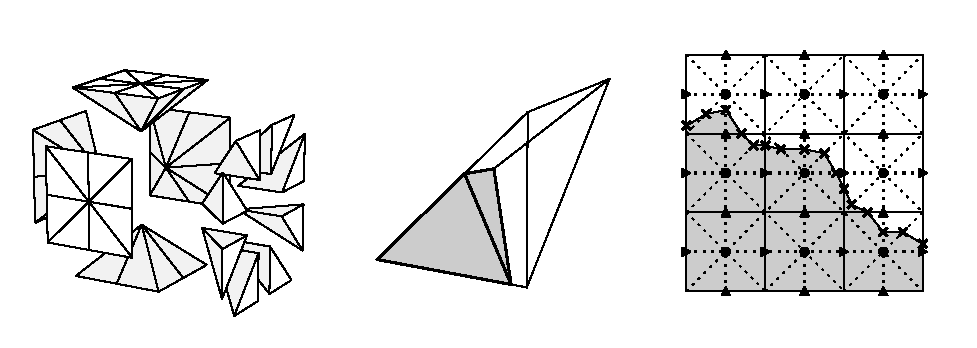
\includegraphics[width=1.0\textwidth]{tetrahedral_scheme}

\begin{itemize}
\item Where the core-environment boundary is determined by interpolating
$q_v$, $q_s$, $T_v$ and $w$.
\end{itemize}
\end{frame}


\begin{frame}
\frametitle{Good agreement between Romps and tetrahedral}
\begin{overpic}[tics=20,width=0.7\textwidth]{direct_vs_romps}
\put(100,80){
\begin{minipage}{0.5\textwidth}
$E_d$, $D_d$
\end{minipage}
}
\put(100,35){
\begin{minipage}{0.5\textwidth}
$\epsilon_d$, $\delta_d$
\end{minipage}
}
\end{overpic}

but there's some dependence on numerics (\small note advection scheme differences)
\end{frame}

\begin{frame}
\frametitle{The tetrahedral technique requires high resolution $\ldots$}
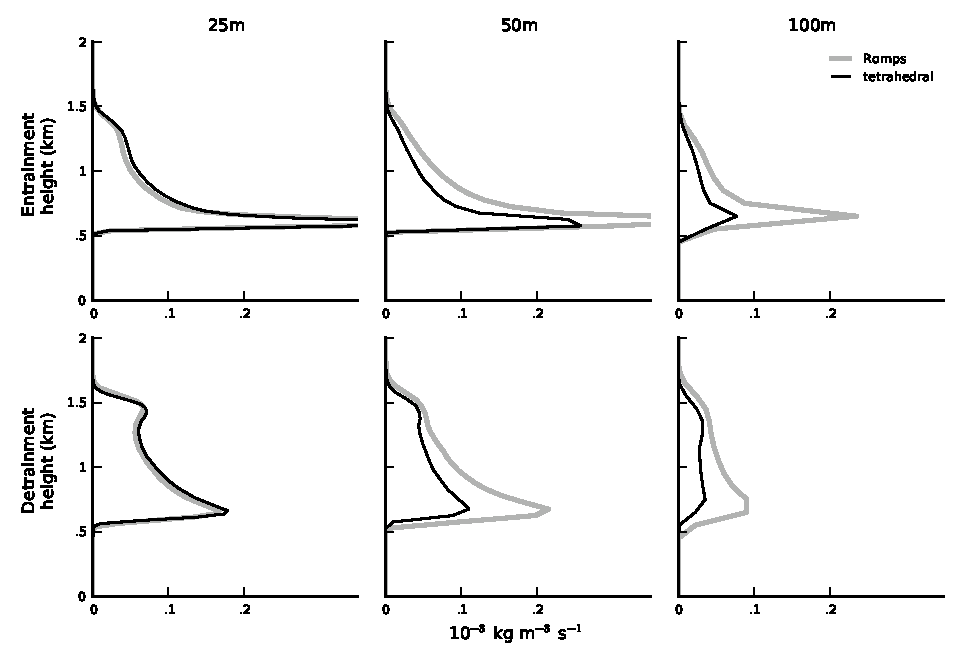
\includegraphics[width=1.0\textwidth]{resolution_dependence}
\end{frame}

\begin{frame}
\frametitle{Because the interpolation biases single gridcell cloud area}
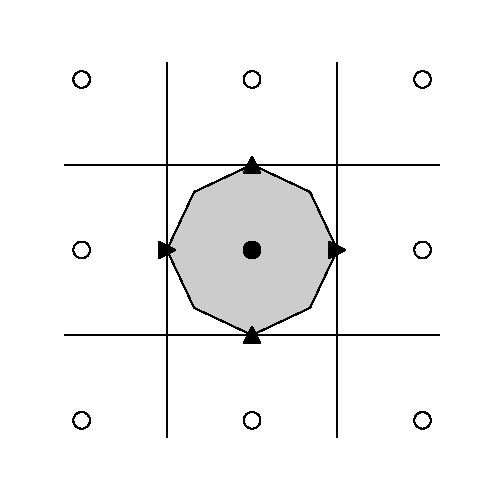
\includegraphics[width=0.8\textwidth]{interpolation_bias}
\end{frame}


\begin{frame}
\frametitle{Tetrahedral fluxes can be used for $E_d/D_d$ snapshots}
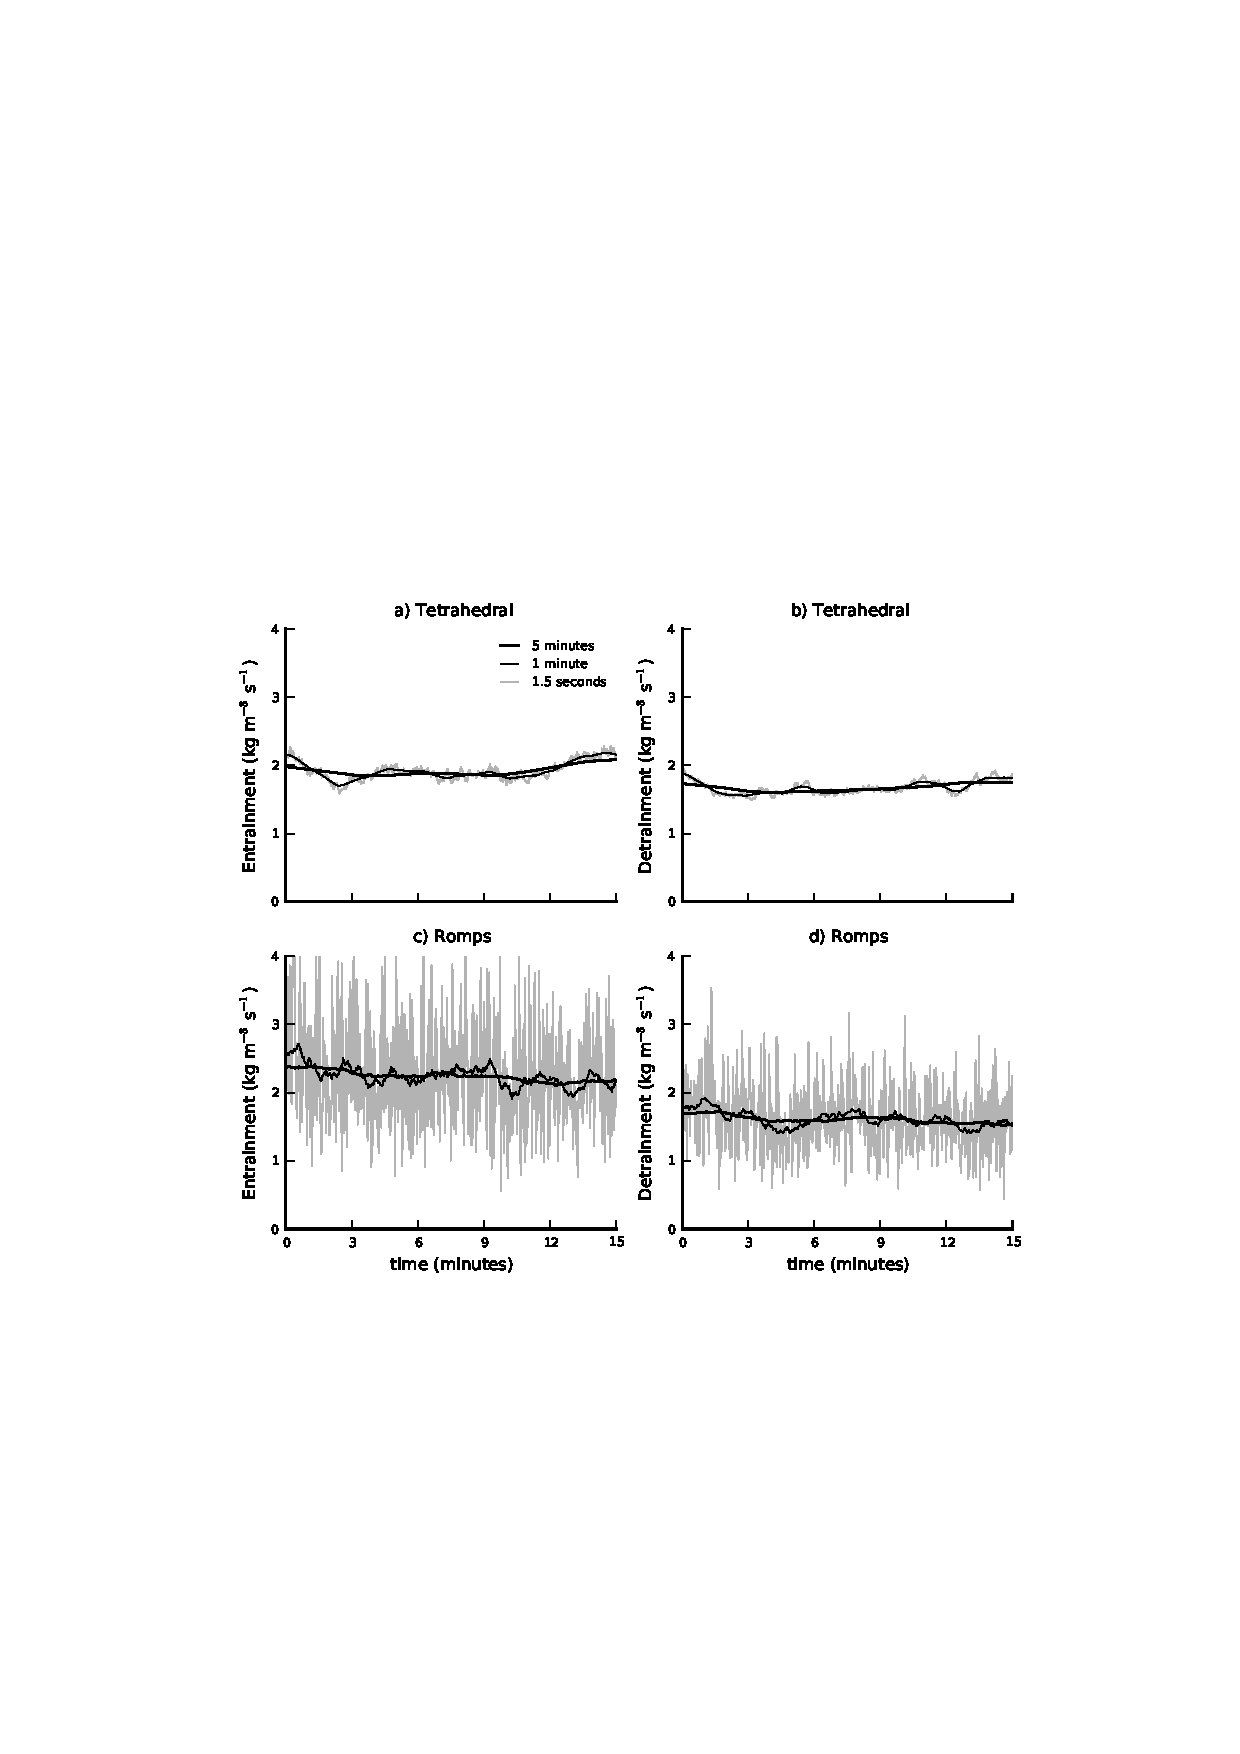
\includegraphics[width=1.0\textwidth]{averaging_convergence.png}
\end{frame}

\begin{frame}
\frametitle{$E_d/D_d$ spatial variability, 1 minute average}

\begin{overpic}[tics=20,width=0.7\textwidth]{spatial_variability_1min.png}
\put(100,80){
\begin{minipage}{0.5\textwidth}
Tetrahedral
\end{minipage}
}
n\put(100,35){
\begin{minipage}{0.5\textwidth}
Romps
\end{minipage}
}
\end{overpic}
\end{frame}

\section{Linking direct and bulk entrainment}
\label{sec:linking-direct-bulk}


\begin{frame}
  \frametitle{Linking direct and bulk entrainment rates}
\includegraphics[width=\textwidth]{mass_radius.jpg}

\mbox{Core:  $w > 0$, $\Delta T_v > 0$, $q_l > 0$}\\
\mbox{Edge: outermost core gridcell}\\
\mbox{Shell: Innermost environment gridcell}

\end{frame}

\begin{frame}
\frametitle{converting $E_d$ to $E_\phi$}
\begin{overpic}[tics=20,width=0.5\textwidth]{reynolds_correctionA}
\put(82,50){
\begin{minipage}{0.5\textwidth}
Define shell and edge tracer values $q_{shell}$ and $q_{edge}$.

These values will differ\\
from $q_c$ and $q_e$, the \\
mean cloud core and environment vapor values

Can show that:

\vspace{-20pt}  
\begin{equation*}
\begin{lgathered}
    E_{\phi} = E_d - E_d\frac{q_{shell} - q_e}{q_{c} - q_{e}}\\
             - D_d\frac{q_c - q_{edge}}{q_{c} - q_{e}}
\end{lgathered}
\end{equation*}

Alternatively, use conditional averages to include Reynolds
correlations

\vspace{-20pt}  
\begin{equation*}
  \begin{lgathered}
  q_E = (E \phi)_d/E_d\\
  q_D =  (D \phi)_d/D_d
  \end{lgathered}
\end{equation*}



\end{minipage}
}

\end{overpic}


\end{frame}




\begin{frame}
\frametitle{Corrected fluxes restore bulk tracer profile}
\includegraphics[width=0.8\textwidth]{reynolds_correctionBC}

The $q_E$ / $q_D$ underestimate of $E$ and $D$ arises from differencing two large quantities:
$q_c(E_d-D_d)$ and $(E q)_d - (D q)_d$. 

\end{frame}



\begin{frame}
\frametitle{Vertical momentum}
\begin{overpic}[tics=20,width=0.5\textwidth]{w_profile}
\put(82,50){
\begin{minipage}{0.5\textwidth}
When we  modify the entrainment calculation
to account for negative and positive $w$,
we find $w_E$, the Reynold's correlated
mean entrained vertical velocity $> 0$ and
nearly as large as $w_D$.

\end{minipage}
}

\end{overpic}


\end{frame}

\begin{frame}
  \frametitle{Why is is the cloud entraining positive $w$?}

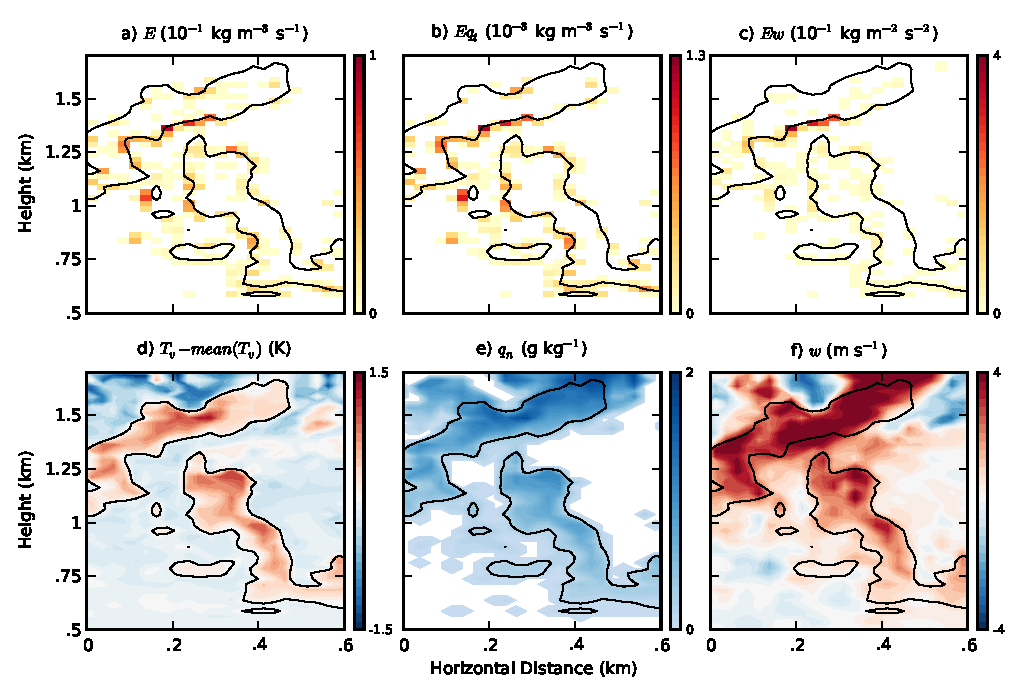
\includegraphics[width=\textwidth]{w_entrainment_example}

Updrafts produce newly buoyant parcels well above cloudbase.
\end{frame}


\section{Summary}
\label{sec:summary}


\begin{frame}
  \frametitle{ Summary}

  \begin{itemize}
  \item Two new techniques to  directly calculate entrainment show
entrainment rates roughly two times higher than bulk values. \pause
\item Much of the difference between bulk and direct calculations is
due to the influence of the heterogeneous cloud shell/edge, but
Reynolds correlations also play a significant role, particularly
for momentum (see our JAS submission) \pause
\item Tetrahedral interpolation can be applied to individual clouds,
and rapidly changing boundary layers, 
either over a cloud life cycle or in a snapshot. \pause

\item The interpolation technique is applicable in general to any
flow through a material surface in a three-dimensional model.

  \end{itemize}

\end{frame}


\begin{frame}
  \frametitle{Thanks to:}

  \begin{itemize}
  \item Marat for providing SAM
  \item Support from the Canadian Foundation for Climate and Atmospheric Science
  \end{itemize}

\end{frame}


\begin{frame}
\frametitle{Romps - tetrahedral correlation}
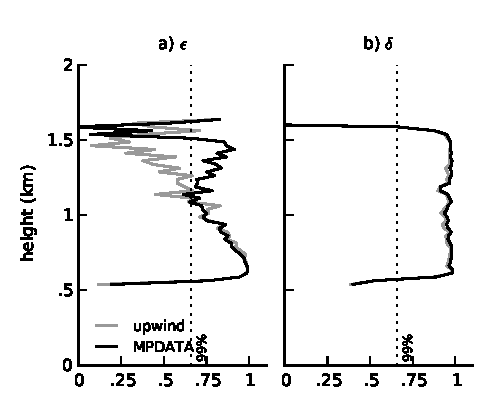
\includegraphics[width=0.8\textwidth]{correlations}
\end{frame}


\begin{frame}
\frametitle{static energy}
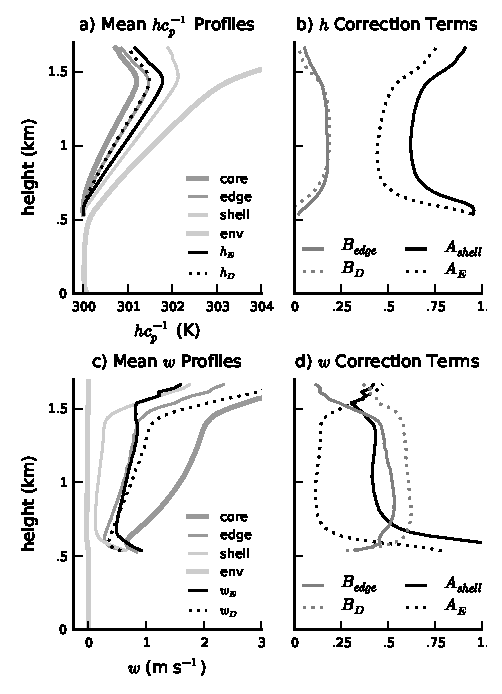
\includegraphics[width=0.4\textwidth]{profile_plots}
\end{frame}


\begin{frame}
\frametitle{ARM diurnal}
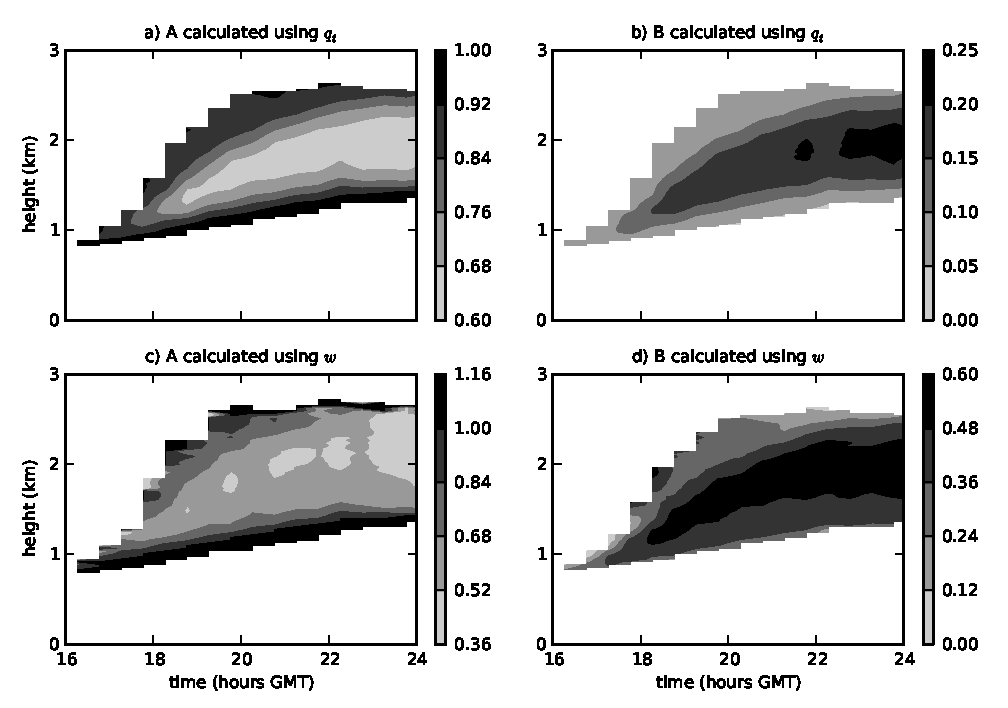
\includegraphics[width=0.5\textwidth]{shell_variability}
\end{frame}


 \end{document}








